\documentclass[10pt,twocolumn]{article} 

% required packages for Oxy Comps style
\usepackage{oxycomps} % the main oxycomps style file
\usepackage{times} % use Times as the default font
\usepackage[style=numeric,sorting=nyt]{biblatex} % format the bibliography nicely
\usepackage{amsmath, amsthm, amssymb, amsfonts}
\usepackage{amsfonts} % provides many math symbols/fonts
\usepackage{listings} % provides the lstlisting environment
\usepackage{amssymb} % provides many math symbols/fonts
\usepackage{graphicx} % allows insertion of grpahics
\usepackage{hyperref} % creates links within the page and to URLs
\usepackage{url} % formats URLs properly
\usepackage{verbatim} % provides the comment environment
\usepackage{xpatch} % used to patch \textcite

\bibliography{references}
\DeclareNameAlias{default}{last-first}

\xpatchbibmacro{textcite}
  {\printnames{labelname}}
  {\printnames{labelname} (\printfield{year})}
  {}
  {}

\pdfinfo{
    /Title (Comps Proposal)
    /Author (Caleb Jordening)
}

\title{DRL in RL: Deep Reinforcement Learning to Train an Agent to Play Rocket League}
\author{Caleb Jordening}
\affiliation{Occidental College}

\begin{document}

\maketitle

\section {Problem Context}

In the past few years, artificial intelligence (AI) has garnered quite the popularity from the media. From self-driving cars to smart-homes and virtual assistants, the future is quite hopeful for all of the technological innovations this field has to offer. Moreover, the sub-category of AI known as deep learning is using neural networks to help in the endeavor of reverse engineering the brain. These artificial neural networks can provide a model to let us understand more about how the biological brain works; and, hopefully, will allow us to produce general AI that possesses cognitive abilities greater than or equal to a human's. Currently, however, we are only able to produce narrow AI that can only perform a single task. 

\subsection{Search for General AI}
In the search for creating general AI, board games and video games provide a high-dimensional, goal-oriented environment in which learning algorithms can be implemented to achieve the goal of the game. Games provide a structure that allows for learning algorithms to be implemented so that the AI can become more adept to learning, which could then potentially generalise to real life applications — resulting in the emergence of general AI. The three most prominent methods for machine learning are: supervised learning, unsupervised learning, and reinforcement learning. Of these three, reinforcement learning is arguably the best suited for training an agent to play a game. Board and video games possess states, rewards, and actions. A person playing the game provides certain inputs that result in actions in the game. Actions are performed to reach a particular state of the game; which, in turn, might provide some sort of reward (points, items, experience, strategic advantage, etc.). Reinforcement learning provides a means by which the agent can be trained by interacting with the world, and seeing what actions lead to the most reward. However, this is not without challenge.

\subsection{Challenges to Machine Learning}
What is known as the "curse of dimensionality" poses a significant obstacle for machine learning development \cite{karanam_2021}. As the number of inputs to be considered increases, the amount of decisions the machine has to filter through in order to find the most optimal action increases exponentially. The more complex a game is, learning becomes a more computationally expensive process. Additionally, the higher-dimensionality created by many inputs can make the most optimal action ambiguous for the machine. High dimensionality can be reduced to a lower-dimension. If this is done, then the problem becomes figuring out a way to shape reward functions in a meaningful way without losing any important information necessary for maximizing the reward.



\section{Technical Background}

\subsection{Reinforcement Learning}
The principles of machine reinforcement learning are extremely similar to how humans learn by interacting with their environment. These interactions provide copious amounts of information about cause and effect relationships; and, this learned knowledge affects decision making and behavior in one's pursuit of achieving their goals. Reinforcement learning provides a computational means by which machines can learn how to achieve certain goals by interacting with their environment via rewards and punishments \cite{Sutton1998}. 

\subsection{Deep Reinforcement Learning}
In 2015, Mnih et al.(2015) \cite{mnih2015humanlevel} created what they called a Deep Q Network (DQN) that implements a deep neural network within a reinforcement algorithm to play Atari video games. This technique was revolutionary, and the reinforcement learning agent was able to outperform humans and other basic reinforcement learning agents in many of the Atari games played. However, DQN was far from a perfect technique – as it struggled with stability issues and was “poorly understood” at the time \cite{DBLP:journals/corr/SchulmanWDRK17}. This instability came from what may be considered the “deadly triad” of deep reinforcement learning, which consists of function approximation, bootstrapping, and off-policy training \cite{https://doi.org/10.48550/arxiv.1812.02648}. DQN happens to exhibit this deadly triad through the incorporation of a DNN, its policy iteration methods, and by learning from data from previous policies – which causes it to diverge from optimal learning policies. Hence, there was a dire need for a data efficient way of implementing deep learning without suffering from divergence.

This led to the creation of the trust region policy optimization (TRPO), which was a gradient policy method that actually worked well in tackling some of these issues. However, this method was too complex and did not scale well to large models \cite{DBLP:journals/corr/SchulmanWDRK17}. Thus, the principles of TRPO were optimized to scale to large models by OpenAI through a policy gradient method called proximal policy optimization (PPO). PPO simplifies the complexities of TRPO and is extremely good at ensuring large updates do not make the policy unstable. Hence, this policy gradient method is one of the most popular DRL policy optimization algorithms to exist at the moment. Additionally, the algorithm works extremely well at performing in complex, continuous environments.


\subsection{Proximal Policy Optimization Algorithm}
\begin{equation}
    \mathop{\hat{\mathbb{E}}}\left [ \textrm{min}\left ( r_{t}(\theta) \hat{A}_{t}, \textrm{clip}\left ( r_{t}(\theta), 1-\epsilon, 1 + \epsilon \right )\hat{A}_{t} \right )\right]
\end{equation}



In general, it is important to note that policy gradient methods function by computing a complex
approximate multi-dimensional policy gradient on which gradient ascent is performed. Ideally,
the objective is to take steps up the gradient in the direction of a certain goal. Taking steps that
are too small will take a long time to converge to the optimal policy. Too large of steps could
lead to falling off of the gradient and negative learning could begin to occur. PPO provides a trust region to limit step sizes. This is done by clipping the policy update region to a small range
denoted by: $\textrm{clip}\left ( r_{t}(\theta), 1-\epsilon, 1 + \epsilon \right )$. In this, epsilon is a hyper parameter that must be chosen to limit how big of an update the policy can take. The advantage, $\hat{A}_{t}$, is a measure of how
different a new action is compared to the on policy action that should be taken. This is calculated
by taking the current Q(s,a) values and subtracting it from an average for all the Q-values
denoted by V(s). $r_{t}(\theta)$ represents the policy ratio of the new policy over the old policy. The
min function ensures that the safest update possible is taken – as taking the max would select the
higher bound which creates a higher risk of instability.

\subsection{Visualizing the Clip}

The plot in Figure 1 shows the clipping process when the advantage value is positive and negative.
The x-axis is the r-value/ratio of the current policy being learned and the baseline policy obtained
through experience. The red dot on both graphs indicate the point at which the advantage would
just be used for an update. The main takeaway from these two graphs is that it shows how the policy updates are very limited in how large of a step they can take given the magnitude of the
ratio between old and current polices and a positive or negative advantage.


\begin{figure}
    \centering
    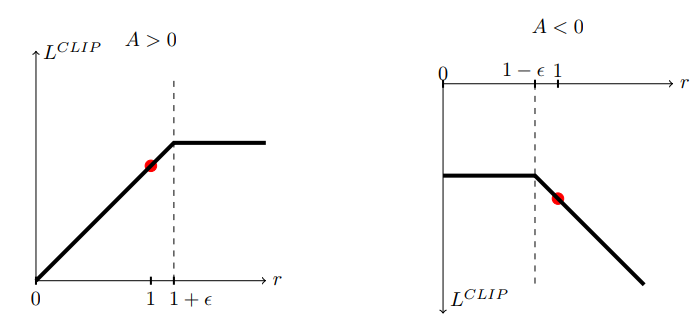
\includegraphics[width=80mm,scale=1]{PPO Clip.png}
    
    \caption{Clip Function Limiting the Size of the Step Taken \cite{DBLP:journals/corr/SchulmanWDRK17}}
    \label{fig:my_label}
\end{figure}

\subsection{PPO in Rocket League}
Ultimately, PPO is a simplification of policy gradient methods that seek to mitigate the problems found in DRL algorithms. While trying to compute an update, PPO’s parameters are simple to tune
– making it scalable to larger models. Each step that is taken minimizes the cost function while
ensuring that the new policy does not deviate from the previous policy too much. This provides
confidence that a policy update will not take too large of a step and fall off of the gradient cliff
and exhibit negative learning. In doing so, the algorithm reasonably chooses step sizes – which,
in turn, allows for much success within continuous environments such as Rocket League.

\section{Prior Work}
The use of reinforcement learning in video games is not a novel idea. A machine called "AlphaGo" was trained via reinforcement learning to play the game Go. In terms of complexity, Go is "profoundly complex" with more possible game configurations than there are known atoms in the universe \cite{deepmind}. \textcite{deepmind} states that prior to their machine, AI was only able to play at the amateur level. After thousands of games of playing against itself, through reinforcement learning, AlphaGo was able to sweep a professional Go player 5-0 in 2015. Later, it was able to beat the world's best Go player. OpenAI Five is another machine that was trained via reinforcement learning to play the game Dota 2\cite{OpenAI_dota}. Dota 2 is a 5v5 battle-arena video game, that involves teamwork in order to achieve victory. OpenAI Five was trained for 180 years per day on 256 GPUs and 128,000 CPU cores. In 2019, OpenAI Five swept a world champion Dota 2 team 2-0. This agent was trained on a complex Deep Reinforcement Learning model that incorporated a long short term memory neural network in it.
\subsection{RLBot}
For the game of Rocket League, Psyonix had developed four levels of AI: "Beginner," "Rookie," "Pro," and "All-Star." The highest level of bot, All-Star, is equivalent to the rank of silver in Rocket League, which is the second lowest rank in the game. This was unfortunate because, as players got better than these bots, there really were no challenges or opportunities to practice in low-stakes environments to further improve. This inspired the RLBot framework to be developed. RLBot enabled programmers to hard-code their own bots using an understanding of the physics and mathematical principles of the game. This allowed for the creation of much better bots; however, these bots could reach nowhere near any of the top competitive ranks.

\subsection{RLGym}
Then came along the Python API called RLGym. Using a Rocket League mod called BakkesMod, RLGym was able to turn Rocket League into an OpenAI gym environment. This allowed for users to train bots via reinforcement and deep reinforcement learning. Due to the high dimensionality and infinite action space full of rich, spatiotemporal data, AI developers are optimistic about utilizing RLGym for machine learning within the game of Rocket League \cite{inproceedings}.

\subsection{Tutorial Bots}
The machine learning community within Rocket League is relatively small; so, aside from the RLGym documentation itself, there is not much literature as to what methods work well, or how to even get started. Recently, Youtuber "Impossibum" released two quick-start tutorials that give a decent baseline for beginning to train an agent; however, the tutorial is limited and uses default libraries and methods to reward shape, create observation builders, etc. Within the tutorial, it is explicitly stated that training an agent for a considerable amount of time on multiple instances will only generate a bot that is "rookie level." It was also stated that there is much room for customization to perhaps create more complex bots.

\subsection{Nexto: The Best Rocket League Bot}
Currently, the best Rocket League "community bot" is called Nexto. It is trained via deep reinforcement learning using the computational power of many people within the Rocket League community. This bot's predecessor, "Necto," was determined to be around the high diamond rank \cite{github}. The team took what they learned from Necto and started fresh in training Nexto. This resulted in Nexto reaching what is considered low grand champ 1 rank, which is 2 ranks above Necto. While it is currently not explicit how long Nexto has trained, there is a gif on the Necto Github repo that says Necto (at one point) had been trained for 9 years, 9 weeks, and 3 days. Necto also won the 2022 RLBot championship by a considerable margin each game.

\section{Methods}

\subsection{Understanding the Tools}
The RLGym API is an adaptation of OpenAI's gym environment, so any of the common reinforcement learning libraries are supported. To make improvements from the tutorial bot, it is imperative that I understand the tools that are available and consider how they could be implemented for my model. This leaves a considerable amount of research and practice to get used to the jargon and fundamentals of reinforcement and deep learning using Python. Specifically, I believe it would be beneficial learn about the Keras API and look at the CartPole-v0 problem to get comfortable with DRL and PPO. Having this understanding would give me a better understanding of the possibilities and limitations of the project itself.

\subsection{Creating a Hard-Coded Bot}
People of the RLGym community strongly suggest that one hard-codes a bot before getting into the reinforcement learning scene. I believe that this would be highly beneficial to do over summer while also learning about Keras. Hard-coding a bot will help me learn about the mathematics and physics of the game. In doing so, I would be able to quantify important data used in the custom observation builder that would be passed to the agent at each state. For example, learning how to describe mathematically where the boost pads are on the map would be important data to pass along to the model during training. 

\subsection{Custom Reward Shaping}

One area that I am particularly interested in for my Rocket League agent is creating custom rewards to help reduce the high-dimensionality of the action space into a lower-dimensional manifold. Custom rewards would be built using knowledge of the domain to help guide the agent towards optimal behaviors and improve training efficiency and potential for generalization \cite{DBLP:journals/corr/abs-1908-06884}. While a large portion of the model's success is dependent on the computational power and amount of time the model is trained, reward shaping could potentially be an area that speeds this process up so that more optimal and intelligent behaviors are observed in a shorter amount of training time. Currently, I am in the 0.10 percent of players in the world sitting at the rank of Grand Champ 2. I follow the Rocket League Esports scene and am aware of current strategies  

\subsection{Custom Observation Builders}

From the tutorial, the advanced observation builder default was used in training the model. This was described as "not that advanced" and a "good default" for starting to build an agent. The tutorial suggests that more complex, custom observation builders can be coded that can provide more useful data about the environment that will be passed to the agent at each new state. Creating custom observation builders is an area in which the overall bot performance and training could be improved.

\subsection{Neural Network Architecture}
Additionally from the tutorial, changes to the neural network architecture were made; however, they were not clearly explained. The same can be said for the tuning of the hyperparameters. Again, this emphasizes the importance of researching the fundamentals and looking at how architecture affects overall performance. From this research, I would be able to analyze and experiment with potential ways in which the architecture could designed to optimize the model's performance. 

\subsection{Training the Agent}

Training the agent will require a lot of computational power and time; and, while I do love my 3060 GPU, I do not believe that this will be sufficient if I want to train multiple models and compare their performance after a certain amount of steps. Ideally, I will use Oxy's cluster to help aid in the computational power that I am lacking to help speed up the process. Additionally, it will allow me to gather the necessary data that I need for model performance comparison given different rewards, observation builders, neural network architecture, etc. 

\section{Evaluation}

\subsection{Model Metrics}
Tensorboard will be used to analyze how the neural network is performing, and to gauge whether or not the model is minimizing the loss while maximizing the reward. These metrics will be assessed in light of how the agent actually performs in matches. 
\subsection{Intelligence, Wins and Losses, Point Breakdown}
Evaluation would occur both qualitatively and quantitatively. Game play would be observed for intelligent behaviors. This could be chasing after the ball, hitting the ball, rotating from offense to defense and vice versa, etc. The bot would also be judged off of whether or not it won or lost the game. Finally, The actual point breakdown would be assessed to see how many saves, epic saves, shots on goal, goals, and ball touches were made. The bot would also be assessed against multiple opponents that vary in skill level. Models will also be trained against other models that were trained by me that have different neural architectures, reward functions, and other potential differences that might help me converge upon training settings that would help me produce the best bot possible. Finally, pending the results of the training and findings, the bot could be tested against low-skilled human players as well. At minimum, the goal is to create a bot that exhibits some sort of intelligent behavior that demonstrates it learned how to somewhat play the game. 


\section{Ethical Considerations}
Implementing deep reinforcement learning within the video game Rocket League does not need to account for too many ethical considerations; however, the use of such algorithms within the real world does. Problems that arise from DRL machines within complex video game environments can actually help foreshadow some of the issues that might arise in a larger scale setting. Ultimately, it is imperative that we take time to make ethical considerations about how such technology might affect society and what precautions may be taken in order to mitigate the possible detriments.

As researches make advances in Artificial Intelligence, governments, organizations, and the general public seek to understand and implement this technology into everyday life \cite{SchiffBBL20}. A popular and promising subset of AI known as Deep Reinforcement Learning (DRL) has greatly contributed to the pervasive hype around AI and its possibilities. With the rapid growth in popularity and progress, it is important to consider the societal and ethical implications that such technology imposes for the future. Studies have already shown how the implementation of AI has resulted in racism/discrimination, algorithmic bias, technological unemployment, and many other challenges that researches must circumvent in hopes of creating an equitable and ethical future \cite{SchiffBBL20}.

\subsection{Data Collection Issues}

To reiterate, the methods of trial-and-error used in DRL to learn optimal policies cannot be used in high stakes settings. Collecting data to find the optimal policies for creating cogent texts through NLPs, making clinical decisions, making money in the stock market, or creating self-driving cars would require performing trial-and-error experiments at the potential cost of being offensive, losing money, and even at the cost of human lives. A machine cannot blow through a stoplight and cause a car accident, make an awful trade that loses a large part of one's portfolio, generate profusely offensive text, or prescribe a treatment to someone that ends up killing them before the machine learns to stray away from such bad behaviors. \cite{10.1613/jair.1.12360}. Simulations may provide environments for training; however, they may not be complex enough to learn and account for every nuance of everyday life. Data collection may also be expensive to obtain, or may infringe on people's privacy. Thus, some parameters may be overlooked or excluded by the machine — leading to more unintentional consequences or discrimination.

\subsection{Reward Hacking}
In the same vein exists the issue of reward hacking by the machine. Much like humans, machines will exploit shortcuts to maximize gain when they are available. If a DRL machine explores and finds a policy that maximizes a reward, it will perform those actions of the policy regardless of whether or not it actually achieves the intended goal. In a real world, high stakes setting, there is no room for error. Especially as objectives become more nuanced and pose high-dimensional problems, reward shaping becomes exponentially more complex; and, there exist more opportunities for the machine to find ways to exploit rewards via a means that do not achieve the desired goal \cite{frye_2021}.

\subsection{DRL in Competitive Rocket League}
Ethical concerns begin to rise as DRL Rocket League bots become better trained. Rocket League is a competitive Esport that has large cash prizes for many of the major tournaments. Outside of the professional scene, there is also a ranked game mode in which many people grind to achieve the highest rank of Supersonic Legend and make their way onto the top leader boards. When these DRL agents surpass the abilities of human Rocket League players, they may find themselves being abused in ranked matches and perhaps could be used to help boost players to higher ranks that they do not actually deserve. In this regard, if these agents were able to enter the competitive scene without others being explicitly aware of their presence, it would ruin the integrity of the game; and, negate the dedication of players who are trying to make the ranked climb earnestly. In an extreme case, someone might figure out a way to have agent play for them in the Esports scene to help them win major tournaments. Again, this would ruin the integrity of the game, and the individual using the unfair agent would essentially be stealing money from the tournaments.

\section{Proposed Timeline}
\begin{itemize}
    \item June 1st: Hard-Code Rocket League Bot
    \item June 15th: Hard-Code Rocket League Bot
    \item July 1st: Vacation
    \item July 15th: Keras Research and Cartpole Problem
    \item August 1st: Keras Research and Cartpole Problem
    \item August 15th: Planning out how to implement what I learned into my project
    \item September 1st: Begin writing out code, draw out architecture
    \item September 15th: Coding
    \item October 1st: Coding
    \item October 15th: Optimizations, Training, Evaluations
    \item November 1st: Optimizations, Training, Evaluations
    \item November 15th: Optimizations, Training, Evaluations
    \item December 1st: Optimizations, Training, Evaluations and begin writing paper
    \item December 5th: Poster presentation
    \item December 15th: Final paper and code due

    
    
\end{itemize}


\printbibliography 

\end{document}
